% Chapter 4

\chapter{Kỹ thuật thu thập dữ liệu} % Main chapter title

\label{Chapter4}
\section{Smart BK Traffic}
Sau quá trình tìm hiểu ngắn, nhóm nhận thấy hệ thống Smart BK Traffic cung cấp một số API để có thể lấy được dữ liệu về tình trạng giao thông thành phố Hồ Chí Minh tại thời điểm sử dụng. Trong đó, API quan trọng nhất được nhóm sử dụng là:
\begin{itemize}
    \item \textit{https://traffic.hcmut.edu.vn/hcm/rest/tc/init?} với các tham số truyền vào là tọa độ của 4 góc bản đồ cần lấy dữ liệu và độ zoom của map, cụ thể là:
\begin{itemize}
    \item latTL, lonTL: vĩ độ, kinh độ của điểm góc trên cùng bên trái
    \item latTR, lonTR: vĩ độ, kinh độ của điểm góc trên cùng bên phải
    \item latBL, lonBL: vĩ độ, kinh độ của điểm góc dưới cùng bên trái
    \item latBR, lonBR: vĩ độ, kinh độ của điểm góc dưới cùng bên phải
    \item zoom: độ zoom của bản đồ
\end{itemize}
    API trên trả về dữ liệu giao thông ở thời điểm gọi API và có cấu trúc như sau:
\begin{lstlisting}[language=XML]
{
  "segs": [
    {
      "v": "lat1,lon1,lat2,lon2,velocity,description,accuracy,id"
    }
  ],
  "last": boolean,
  "key": "key"
}
\end{lstlisting}
    Trong đó:
    \begin{itemize}
        \item "segs": là một mảng các segment, thông tin mỗi segment được lưu trong field "v" với các thuộc tính được phân cách nhau bằng dấu phẩy:
        \begin{itemize}
            \item lat1,lon1: vĩ độ, kinh độ điểm đầu của segment
            \item lat2,lon2: vĩ độ, kinh độ điểm cuối của segment
            \item velocity: vận tốc trên đoạn segment đó 
            \item description: miêu tả về đoạn segment
            \item accuracy: độ chính xác của giá trị vận tốc
            \item id: id của field "v".
        \end{itemize}
    
    \item "last": có giá trị boolean để xác định segment trả về đã là cuối cùng hay chưa. Nếu chưa thì sẽ có giá trị bằng \textit{false} và tạo ra key ở field "key" để có thể tiếp tục get dữ liệu.
    \item "key": tham số của API \textit{https://traffic.hcmut.edu.vn/hcm/rest/?key=} để get tiếp dữ liệu các segment còn thiếu.
    \end{itemize}
\end{itemize}
Sau khi đã hiểu rõ được cách làm việc của API, nhóm quyết định sử dụng Java Framework Spring Boot kết hợp với OpenStreetMap để tạo ứng dụng web hiển thị bản đồ tình trạng giao thông dựa trên dữ liệu lấy được từ các API trên.

\begin{figure}[!ht]
	\begin{center}
		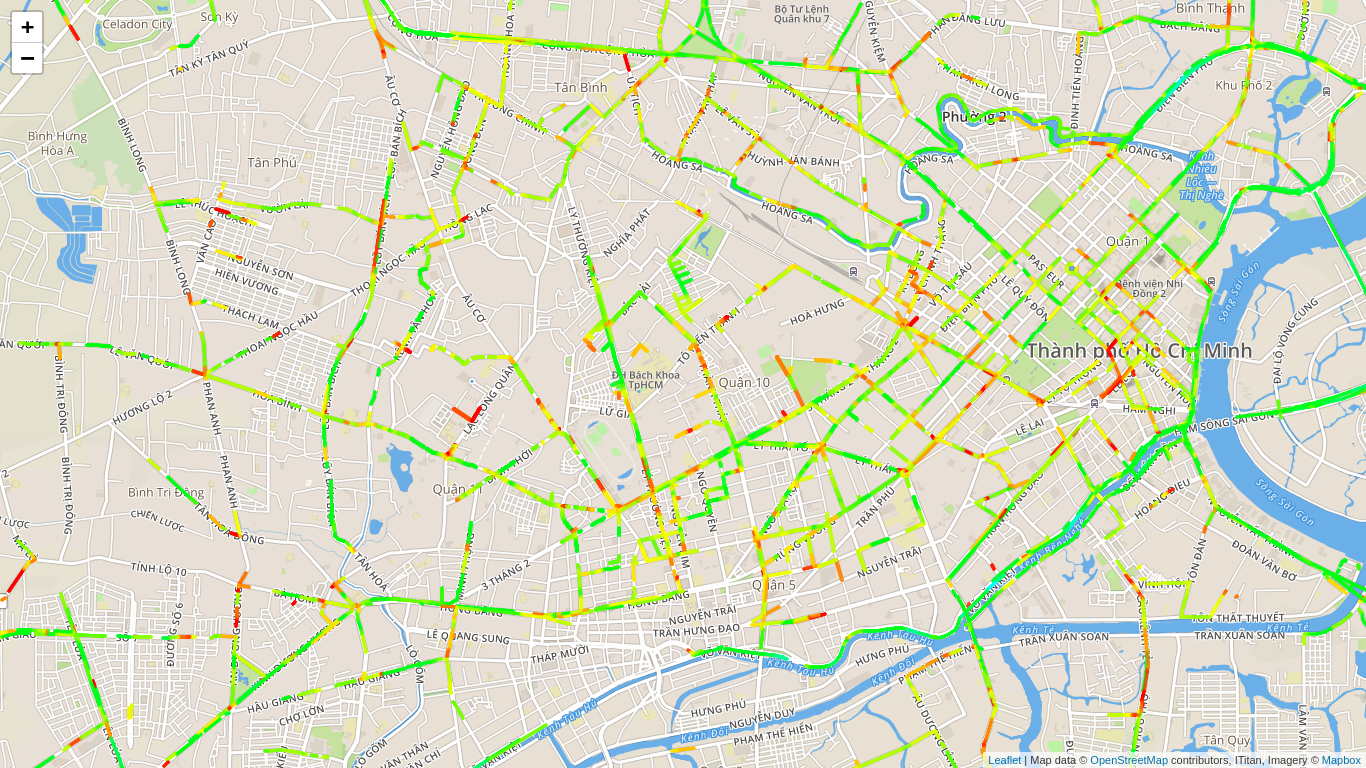
\includegraphics[width=1.0\textwidth]{Traffic_Report/images/map.png}
	\end{center}
	\caption{Web application hiển thị tình trạng giao thông thành phố Hồ Chí Minh}
\end{figure}

Đồng thời, nhóm cũng viết một chương trình nhỏ để lấy dữ liệu toàn thành phố Hồ Chí Minh mỗi 15 phút và lưu xuống database là Mongodb. Để lấy được dữ liệu của toàn thành phố, nhóm xác định bốn điểm tọa độ của vùng bao phủ thành phố và từ đó chia nhỏ ra thành 16x16 vùng nhỏ hơn để có thể thu thập dữ liệu được chính xác hơn. Vì nếu chỉ sử dụng bốn điểm tọa độ của vùng bao phủ thành phố thì API chỉ trả về dữ liệu của một số tuyến đường quan trọng trên bản đồ, dẫn đến sự thiếu sót dữ liệu. Sau khi xác định được các vùng nhỏ để tránh sự thiếu sót dữ liệu, nhóm sử dụng các API trình bày ở trên để thu thập và lưu dữ liệu theo cấu trúc của các model mà nhóm đã thảo luận, thống nhất với hai nhóm làm đề tài giao thông khác. Chi tiết về thiết kế cơ sở dữ liệu sẽ được trình bày ở phần 5.

\section{Dữ liệu từ cộng đồng (Crowdsourcing)}
Ở giai đoạn đề cương luận văn, việc thu thập dữ liệu từ cộng đồng chỉ dừng lại ở những bước xây dựng nền tảng để có thể thực hiện thu thập dữ liệu ở giai đoạn sau. Cụ thể, nhóm tham gia thảo luận với hai nhóm làm đề tài giao thông còn lại và đưa ra các đánh giá, nhận xét để xây dựng mô hình quan hệ thực thể, cũng như đóng góp ....


Xd ứng dụng, thảo luận các pp đánh giá tính xác thực của dữ liệu,

